\section{Experiments}
\label{sec:Experiments}
characterizing the repeatability of one tag


%%%%%%%%%%%%%%%%%%%%
\subsection{Tag Characterization Experiments}

\begin{figure}[H]
	% Data

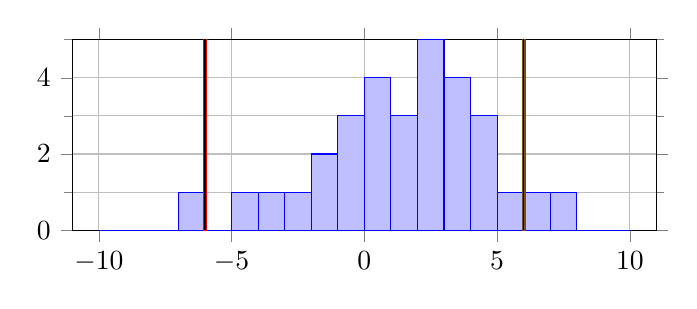
\begin{tikzpicture}
\begin{axis}[
height=4cm,
width=9cm,
%            ybar interval,      % <-- this causes the `xticks' to be centered
ymin= 0, ymax=5,
xmin=-11, xmax=11,
grid=both,
minor y tick num=1,
%yminorgrids=true,
tick align=outside, % <-- this positions the ticks "outside"
]
\addplot+ [
ybar interval,
mark=none,
fill=blue!25,   % fill the bars again
] coordinates {

	(-10,0)	%
	(-9,0)	%
	(-8,0)	%
	(-7,1)	%
	(-6,0)	%1
	(-5,1)	%11
	(-4,1)	%11
	(-3,1)	%111111
	(-2,2)	%11111
	(-1,3)	%111111
	 (0,4)	%11111
	 (1,3)	%1
	 (2,5)	%
	 (3,4)	%
	 (4,3)	%
	 (5,1)	%
	 (6,1)	%
	 (7,1)	%
	 (8,0)	%
	 (9,0)	%
	 (10,1)	%

};

\addplot+ [
ybar interval,
mark=none,
fill=black,   % fill the bars again
] coordinates {
	(-6.05,16) 
	(-5.95,16) 
};

\addplot+ [
ybar interval,
mark=none,
fill=black,   % fill the bars again
] coordinates {
	(6.05,16) 
	(5.95,16) 
};
\end{axis}

\end{tikzpicture}
	\caption{Histogram of one sensor face reading the same tag multiple times}
	\label{fig:histogram}
\end{figure}

We did some stuff, wrote it down here...

%%%%%%%%%%%%%%%%%%%%
\subsection{Crystalization Experiments}

We did some stuff, wrote it down here...


%%%%%%%%%%%%%%%%%%%%
%%%%%%%%%%%%%%%%%%%%
%%%%%%Old Text%%%%%%
%%%%%%%%%%%%%%%%%%%%%
%%%%%%%%%%%%%%%%%%%%%
%%%%%%%%%%%%%%%%%%%%%%
%
%
%This section presents the results of both system-level experiments and
%hardware characterization for the 3D M-Block system.  We performed
%nine sets of lattice reconfiguration experiments, and have recorded
%the success rate of each movement in
%Table~\ref{tab:results}. Additionally, we experimentally measured the
%torque profile of the inertial actuator under several different input
%parameters. The magnetic bonding system was previously characterized in~\cite{RomanishinRus-IROS13}, and has since not undergone significant changes, therefore we
%do not repeat those measurements here. Furthermore, we discuss several
%less formal experiments involving 3D M-Blocks moving independently and
%as assemblies.
%
%\subsection{Lattice Reconfiguration Experiments}
%
%We performed a series of nine representative lattice reconfiguration
%experiments with a single module, as shown in
%Table~\ref{tab:results}. Each reconfiguration movement was tested at
%least twenty times, and the overall success rate for all of the
%motions combined is over 88\%. The success rate has increased for
%every movement as compared to the corresponding experiments in
%~\cite{RomanishinRus-IROS13}, except for the horizontal traverse, and
%the horizontal concave motions, see Table~\ref{tab:results}. The success rates of these motions
%was lower, which we attribute to the higher module weight, and
%interference with the edge teeth while performing rotations of
%$\pi$~radians. Additionally, the modules are now able to perform the
%stair step motion, which requires more torque than the previous M-Blocks
%were able to provide. However, since the pivoting motion exerts
%significant forces and torques on the entire lattice structure, some
%of these motions will not perform as tested under differing lattice
%configurations.  For example, if the lattice contains only a few
%modules, it may be too weak to maintain its structural integrity during
%some transitions, or it may not be massive enough to
%serve as an immobile substrate on which individual modules move.  We
%believe that generic 3D lattice reconfiguration will be possible in
%a system containing many M-Blocks, as long as the motion planner is
%capable of recovering from occasional movement failures.
%
%%%%%%%%%%%%%%%%%%%%%%%% Begin Big Table %%%%%%%%%%%%%%%%%%%%%%%
%\begin{table*}[th]
%  \centering
%    \caption{Experimental results for controlled
%      tests of various motion primitives are shown. A video of some of these experiments can be found under the link in the supplementary materials section.}
%
%  \begin{tabular}{ |p{1.1cm}|p{1.4cm}| p{1.4cm}|p{1.4cm}|p{1.4cm}|p{1.4cm}|p{1.4cm}|p{1.4cm}|p{1.4cm}|p{1.4cm}|  }
%  \hline
%    & Traverse & Horizontal Traverse & Vertical Traverse & Horizontal Convex & Vertical Convex & Horizontal Concave & Vertical Concave & Corner Climb & Stair Step\\
%    \hline
%   Illustration & {\vspace{.1cm}\includegraphics[width=1.4cm]{Figures/motions/motionsa}} &  {\vspace{.1cm}\includegraphics[width=1.4cm]{Figures/horizontaltraverse}} & {\vspace{.1cm}\includegraphics[width=1.4cm]{Figures/verticaltraverse}}   & {\vspace{.1cm}\includegraphics[width=1.4cm]{Figures/horizontalconvexnew}} & {\vspace{.1cm}\includegraphics[width=1.4cm]{Figures/motions/motionsc}} &{\vspace{.1cm}\includegraphics[width=1.4cm]{Figures/horizontalconcavenew}} & {\vspace{.1cm}\includegraphics[width=1.4cm]{Figures/motions/motionsb}}  & {\vspace{.1cm}\includegraphics[width=1.4cm]{Figures/motions/cornerclimb}}  &{\vspace{.1cm}\includegraphics[width=1.4cm]{Figures/motions/stairclimb}} \\
%    \hline
%     Attempted & 41& 20& 20& 20& 20& 20& 20& 20& 20 \\
%    \hline
%     Success &100\% &70\% &80\%  &95\% &100\%  &55\% & 90\%& 100\%&95\% \\
%    \hline
%  \end{tabular}
%  \label{tab:results}    
%\end{table*}
%
%
%%%%%%%%%%%%%%%%%%%%%%%% End Big Table %%%%%%%%%%%%%%%%%%%%%%%
%
%\subsection{Characterizing the Inertial Actuator}
%
%In order to reconfigure the 3D M-Block about a lattice structure, a
%torque is required which is powerful enough to overcome the
%substantial magnetic bonds attaching the module to its neighbors, but
%not so powerful that the module disconnects from the structure
%completely.  The inertial actuator can generate torque through two
%methods: accelerating or decelerating the flywheel electronically,
%or by application of the mechanical brake to the rotating
%flywheel. As shown in Figure~\ref{fig:accel}, the acceleration and the electronic braking of the flywheel generate for a period up to 1\,s maximum
%torques on the order of 0.03\,Nm, and 0.04\,Nm, respectively. While these
%torques are not sufficient to perform any lattice reconfiguration
%movements, they allow the module to locomote independently, and to change
%planes.  The application of the mechanical brake, in contrast,
%generates torques over a much shorter duration (10--30\,ms) but which
%approach a maximum of 2.6\,Nm.  This magnitude of torque allows the
%modules to perform all but the most difficult lattice moves. For
%example, an upward stair-step while connected by four faces (below,
%front, left, and right) is not currently possible.
%  
%  %%%%%%%%%%%%%%%%%%%%%%%%%%% BEGIN Actuator Graph Figure %%%%%%%%%%%%%%%%%%%%%%%%%%%%%%%
%  \begin{figure}[htbp]  
%
%  \centering
%  \includegraphics[width=3in]{Figures/ebrake}
%
%  \caption{This graph shows the torques generated by the inertial
%    actuator through acceleration and electronic braking, without any
%    use of the mechanical brake. These torques are sufficient to move
%    a single module across the ground in an unstructured environment.
%    Additionally, these torques are sufficient to cause the central
%    assembly to change planes when the locking pin is retracted. }
%
%  \label{fig:accel}    
%\end{figure}
%%%%%%%%%%%%%%%%%%%%%%%%%%%% End Actuator Graph Figure %%%%%%%%%%%%%%%%%%%%%%%%%%%%%%%
%
%The mechanical brake generates torque through a self-tightening band
%brake as described in Section~\ref{sec:FlywheelAndBraking}. The
%torques generated by the mechanical brake display inherent variability
%due to variable tolerances of the components amplified 
%bt the non-linear nature of many of the interactions. While we do not have complete control over the resultant
%torque, we do have control over three variables which govern the
%braking event: the flywheel rotational speed (up to 20000\,RPM); the
%current supplied to the brake (up to 4\,A); and brake actuation time (up to 250\,ms).  We have performed an initial
%characterization of the torque generated with the mechanical brake by
%directly measuring  torque for several different input
%combinations using a load-cell based Futek TFF500 torque sensor
%sampling at 10\,kHz (see Figure~\ref{fig:brakegraph}). Although we have
%not explored the complete mapping between all of the inputs and the
%resulting torque, we have determined sufficient input parameters for
%lattice movements through trial and error. Since the values for
%lattice reconfigurations were experimentally determined, the repeatability of an output given the same
%input is important for consistent system performance.  A qualitative sense of the repeatability of the actuator can be seen in
%Figure~\ref{fig:brakegraph}. While Figure~\ref{fig:brakegraph} only
%shows data from a single cube, there is additional variability between the
%actuators of different modules. We hope to eliminate this variability through
%more consistent manufacturing and calibration of each module.
%
% %%%%%%%%%%%%%%%%%%%%%%%%%%% End Actuator Graph Figure %%%%%%%%%%%%%%%%%%%%%%%%%%%%%%%
%
%% We have observed an interesting pattern in the torque, which
%%includes a sudden spike, followed by a period of lower torque for
%%most inputs. We are not sure why exactly the torque profile follows
%%this path instead of a simple triangle shaped graph, but it could be
%%due to a recoil of the brake arm assembly due to the elasticity of
%%the brake assembly, and a very sudden force generated in the initial
%%ramp up of torque during the first few milliseconds of the brake
%%event.
%
%%However, since we use an experimental method to match input
%%parameters to required lattice reconfiguration motions the important
%%is how consistent the torque profile is to a given set of input
%%parameters. One demonstration of the degree of reliability can be
%%seen in the first set of lines in Figure~\ref{fig:brakegraph}, where
%%ten of the maximum input parameters, 10000 RPM, 4000 amps current,
%%250ms brake time are plotted. The maximum values were within a range
%%of $\pm$ 5 percent, and the overall shape appears quite
%%similar. However there are more significant differences between
%%different M-Blocks which are likely due to manufacturing tolerances,
%%which we are currently attempting to solve through improved machining
%%processes.  We have observed an interesting pattern in the torque,
%%which includes a sudden spike, followed by a period of lower torque
%%for most inputs.
%%%%%%%%%%%%%%%%%%%%%%%%%%%%%%%% Actuator Graph Figure %%%%%%%%%%%%%%%%%%%%%%%%%%%%%%%%
%%\begin{figure}[htbp]  
%%
%%  \centering
%%  \includegraphics[width=2in]{Figures/Fixture}
%%
%%  \caption{This fixture attaches an M-Block 3D to the ground through a Futek TFF500 torque sensor. The measurements are captured at 10000hz using a NI USB-6009 DAQ.}
%%
%%  \label{fig:fixture} 
%%\end{figure}
%%   
%%%%%%%%%%%%%%%%%%%%%%%%%%%% End Actuator Graph Figure %%%%%%%%%%%%%%%%%%%%%%%%%%%%%%%%
%
%\begin{figure}[htbp]  
%
%  \centering
%  \includegraphics[width=3in]{Figures/torque_v_rpm}
%
%  \caption{This graph shows the torque generated by the inertial actuator for different input parameters
%    measured at a rate of 10\,kHz. The bold lines represent the mean
%    values of the torque. The 14000\,RPM experiment actuated the brake with 4000\,mA current for 250\,ms, while the 9000\,RPM, and 5000\,RPM experiments actuated the brake for 2000\,mA for 250\,ms. }
%
%  \label{fig:brakegraph}    
%\end{figure}
%
%%%%%%%%%%%%%%%%%%%%%%%%%%%% End Actuator Graph Figure %%%%%%%%%%%%%%%%%%%%%%%%%%%%%%%%
%
%\subsection{Plane Changing}
%
%The plane changing process is under-actuated, (see
%Section~\ref{sec:PlaneChanging}), and we do not have precise control
%over its performance.  In order to change planes, we apply a torque
%using the electronic brake while the locking pin is retracted, wait
%until the internal assembly stabilizes into a position, and then use
%the IMU in order to verify whether the orientation is as desired.  In
%the case that it does not achieve the correct orientation, the module
%continues trying to change planes until the correct orientation is
%achieved. We performed ten experiments where we cycled through desired
%orientations. The module was able to correctly align its orientation
%in all ten attempts, with an average time to do so of 21.7~s,
%with a standard deviation of 17~s. Currently the ability to
%change planes works optimally while the module is attached to a lattice
%structure, although it is still possible while the module is
%independent.
%
%% We are still refining the control software for plane changing and
%% expect the performance to improve significantly in the future.
%
%\subsection{Additional Experiments}
%%%%%%%%%%%%%%%%%%%%%% Big Table %%%%%%%%%%%%%%%%%%%%%
%
%
%In addition to the individual module lattice reconfiguration moves presented
%in Table~\ref{tab:results}, we have tested several movement
%capabilities in a less formal manner. The 3D M-Blocks are able to move
%independently using several motion primitives.  While moving
%independently, 3D M-Block modules are able to move forwards or backwards along the actuator plane
%in steps ranging from a single controlled roll about an edge (50~mm),
%to a more stochastic single movement of up to 1.5~m at full actuator
%power.  Additionally, when the inertial actuator is oriented parallel
%to the ground plane and the motor is quickly accelerated 
%for 1~s, the modules perform a random walk by rolling about their
%corners, and travel a distance of approximately 0.5~m along a random
%heading while coming to rest in a random orientation. Using these
%movements, the 3D M-Blocks should be able to disperse, thoroughly
%explore an environment, and then re-aggregate into a single structure.
%
%Multiple 3D M-Blocks are able to perform lattice reconfiguration
%movements in parallel as a meta-module.  We have performed a proof of
%concept experiment with two modules executing a coordinated
%traverse. However, in order to reliably perform coordinated movements
%we need to further develop the software in order to ensure consistent
%synchronization between modules. Examples of these motions, as well as
%samples of the lattice reconfiguration experiments, can be found in the
%video linked in supplementary materials.
%

